%%% Laboratory	 Notes
%%% Template by Mikhail Klassen, April 2013
%%% Contributions from Sarah Mount, May 2014
\documentclass[a4paper]{tufte-handout}

\newcommand{\workingDate}{\textsc{Dec $|$ 2016}}
\newcommand{\userName}{Felix Engstr\"om}
\newcommand{\institution}{KTH}

\usepackage{lab_notes}

\usepackage{hyperref}
\hypersetup{
    pdffitwindow=false,            % window fit to page
    pdfstartview={Fit},            % fits width of page to window
    pdftitle={Projekt lab notes 2016},     % document title
    pdfauthor={Felix Engstr\"om},         % author name
    pdfsubject={},                 % document topic(s)
    pdfnewwindow=true,             % links in new window
    colorlinks=true,               % coloured links, not boxed
    linkcolor=DarkScarletRed,      % colour of internal links
    citecolor=DarkChameleon,       % colour of links to bibliography
    filecolor=DarkPlum,            % colour of file links
    urlcolor=DarkSkyBlue           % colour of external links
}


\title{Projekt lab notes}
\date{2016}

\begin{document}
\maketitle

%%%%%%%%%%%%%%%%%%%%%%%%%%%%%%%%%%%%%%%%%%%%%%%%%%%%%%%%

\begin{projects}
	\begin{description}
		\item Exploration and implementation of algorithm for classifcation of 
            signal-peptides.
    \end{description}
\end{projects}

%%%%%%%%%%%%%%%%%%%%%%%%%%%%%%%%%%%%%%%%%%%%%%%%%%%%%%%%
\newday{19 december 2016}

We have decided to mainly focus on implementing a classifier using some sort of HMM approach. 
If there is time we will also try to do something using an RNN. The first step will be writing code to handle and import the data.


\newday{20 december 2016}

Today we implemented the first attempt at using an HMM. We used the hiden states from the data to train two models. One on the positive data and one on the negative data. We then used these to score the data points in the test set, chosing the model that had the higthes probability score. 

\begin{figure}
    \begin{center}
      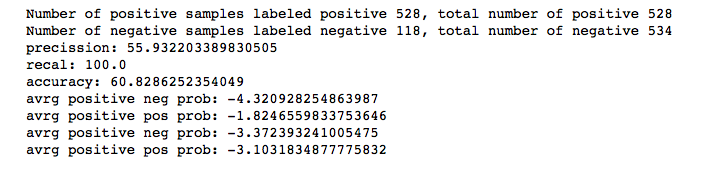
\includegraphics[width=0.8\textwidth]{pics/HMM_old.png}
    \end{center}
    \caption{Results from first run.}
\end{figure}

This approach did not fare so well. It seems that the mean probability of the negative model is much lower, creating a classifier that is overly prone to positive classification.

We will now try a different approach, were we instead train a model on all the samples, and have it predict a hiden state sequence for the given protein sequence. We then use the hiden state sequence to predict the class of the data by looking for "C".

\newday{21 december 2016}

Using the single model approach mentioned earlier

\begin{figure}
    \begin{center}
      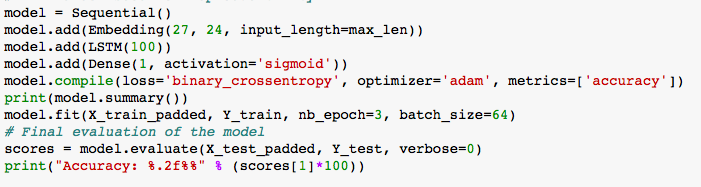
\includegraphics[width=0.8\textwidth]{pics/code_run_1.png}
    \end{center}
    \caption{Code for the first run.}
\end{figure}

This model was trained without dropout and with an embedding layer that was probably unneccesary.
The run took about 2 hours.

\begin{figure}
    \begin{center}
      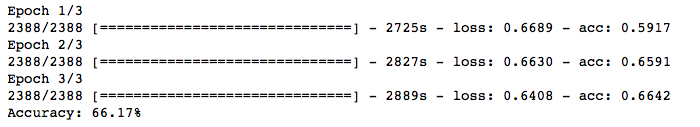
\includegraphics[width=0.8\textwidth]{pics/first_run.png}
    \end{center}
    \caption{Stats from the first run}
\end{figure}

\newday{21 december 2016}

Today we finished an HMM approach to the problem. In this we use the
hidden-state data to create a markow model for all the peptides in the training
data. Then to classify new sequences we use the model to predict the the hiden
state of the sequence, and then look at the produced hiden-state to decide if
the sequence is a signal peptide.

\newday{22 december 2016}

We are now trying to use our model to analyze the proteome. We realized that
our model had no way of handleing errors in the data, or '*' and had to adjust
for this. 

\hrulefill

%%%%%%%%%%%%%%%%%%%%%%%%%%%%%%%%%%%%%%%%%%%%%%%%%%%%%%%%
\bibliographystyle{plain}
\bibliography{lab_notes}

\end{document}
